\begin{comment}
\begin{figure}
\centering
	% To include a figure from a file named example.*
	% Allowable file formats are eps or ps if compiling using latex
	% or pdf, png, jpg if compiling using pdflatex
	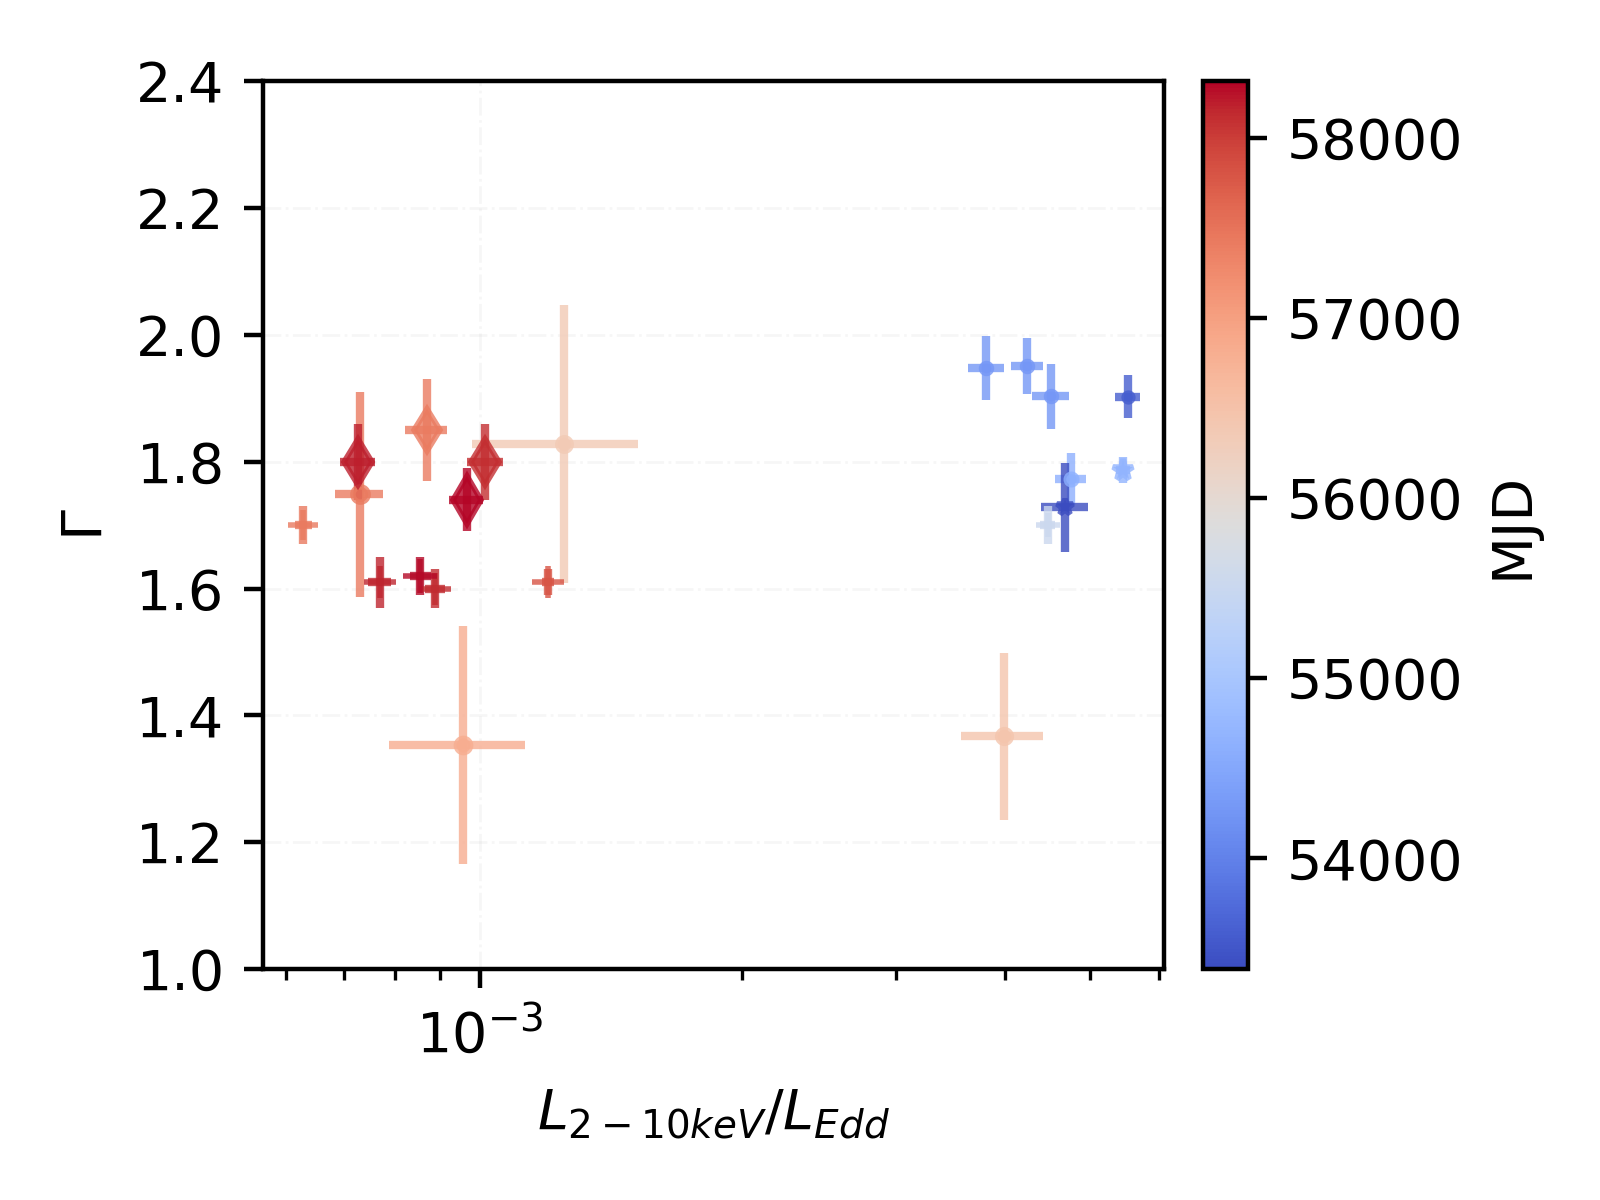
\includegraphics[width=0.7\columnwidth]{./pic/xrayappendgood-eddrate-g-tmap.png}
    \caption{$\Gamma$ and eddington rate evolution}
    \label{fig:xrayappendgood-eddrate-g-tmap}
\end{figure}
\end{comment}

Data of Mrk~590 and NGC~7213 come from \citet{2016MNRAS.460..304K} and \citet{2011MNRAS.411..402B}, respectively. Grey line means the fundamental plane defined in \citet{2003MNRAS.345.1057M}.



%emphasize the importance of multi-wavelength evolution, then introduce the observations in different bands reported previously.
% Thus, multi-wavelength observations provide us an approach to the activities of the central engine of AGNs because the emissions of different wavelengths might originate from different components or different radiation mechanism. 
%For example, the X-ray emission is from the corona, the optical/UV emission is from accretion disk and the radio emission is from jet. 


\citet{1997MNRAS.286..513R} analysed X-ray spectrum of 24 type 1 AGN sampled from the EXOSAT survey of \citet{1989MNRAS.240..833T} and the Ginga survey of \citet{1994MNRAS.268..405N} with 18 Seyfert 1 galaxies and 2 radio-quiet quasars, the others are 3 broad-line radio galaxies and 1 radio-loud quasar. The X-ray spectrum fit based on power-law continuum, Gaussian line, two absorption edges, plus intrinsic and Galactic absorption shows a random distribution in $\Gamma-L_x$ diagram with Spearman's correlation coefficient: 0.25, pvalue: 0.24 and Pearson's correlation coefficient: -0.14, pvalue: 0.52, where the luminosity range from $1.78\times 10^{41}$ to $1.53\times 10^{47} erg s^{-1}$. It is consistent with \citet{2015AASP....5...79S} sampled from 97 Seyfert 1 galaxies, where the luminosity range from $4.5\times 10^{41}$ to $9\times 10^{44} erg s^{-1}$. 


\citet{2008ApJ...682...81S} found the positive correlation between the hard X-ray photon index ($\Gamma$) and accretion rate (L/LEdd) for 35 moderate to high luminosity Radio-Quiet AGNs with z at 1.3$\sim$3.2. They also found that the optical-X-ray spectral slope ($\alpha_{OX}$) depends mainly on optical-UV luminosity, rather than $L/L_{Edd}$, consistent with \citet{2012MNRAS.423..600S} but in Type 1 AGNs at low z(0.005$\sim$0.31) where luminosity mainly drives the X-ray to UV emission ratio , rather than $M_{BH}$ or $L/L_{Edd}$.







Before fading into the faint state, it shows rapid variability in X-ray and optical band. While Mrk~1018 shows strong correlation between UVOT and X-ray band, the flux in UVOT varies more than that in X-ray as a whole but reverses during type transition within short timescale. The type transition timescale for Mrk~1018 is around 2 years(between 2013--2015) or less, while the minimum timescale for variability can be as short as $\sim$ 100 days during transitional phase and several days in the faint state. The photon index($\Gamma$) indicating the hardness in X-ray appears as ``V-shape'' compared to luminosity. We find that $\alpha_{OX}-L_{UV}$ diagram is well linked to type of Mrk~1018 in comparison with another two CL AGNs. However, there is only weak variability in the radio band, which might implies the hybrid mode in accretion or jet process.



\citet{2017ApJ...841L..18M} summarized that as X-ray luminosity increase, the relative fraction of observed Type 2 AGN to Type 1 AGN decreased, even though the median X-ray luminosity is almost equal, where only AGNs with $L_x \geq 10^{42} erg s^{-1}$ and $z \leq 1$ were considered to avoid the host galaxy contamination and evolution effects.

\citet{2018MNRAS.476L..34S} modeled the AGN variability timescale from days to Gyr.

\citet{2019arXiv190800742C} reviewed the basic scenarios where the Broad Line Region (BLR) originate, such as inflow model, formation 'in situ', wind-disk model, etc. 


The luminosity of AGN might drive the emission line and disk-corona in separate ways.



\begin{figure}
\centering
	% To include a figure from a file named example.*
	% Allowable file formats are eps or ps if compiling using latex
	% or pdf, png, jpg if compiling using pdflatex
	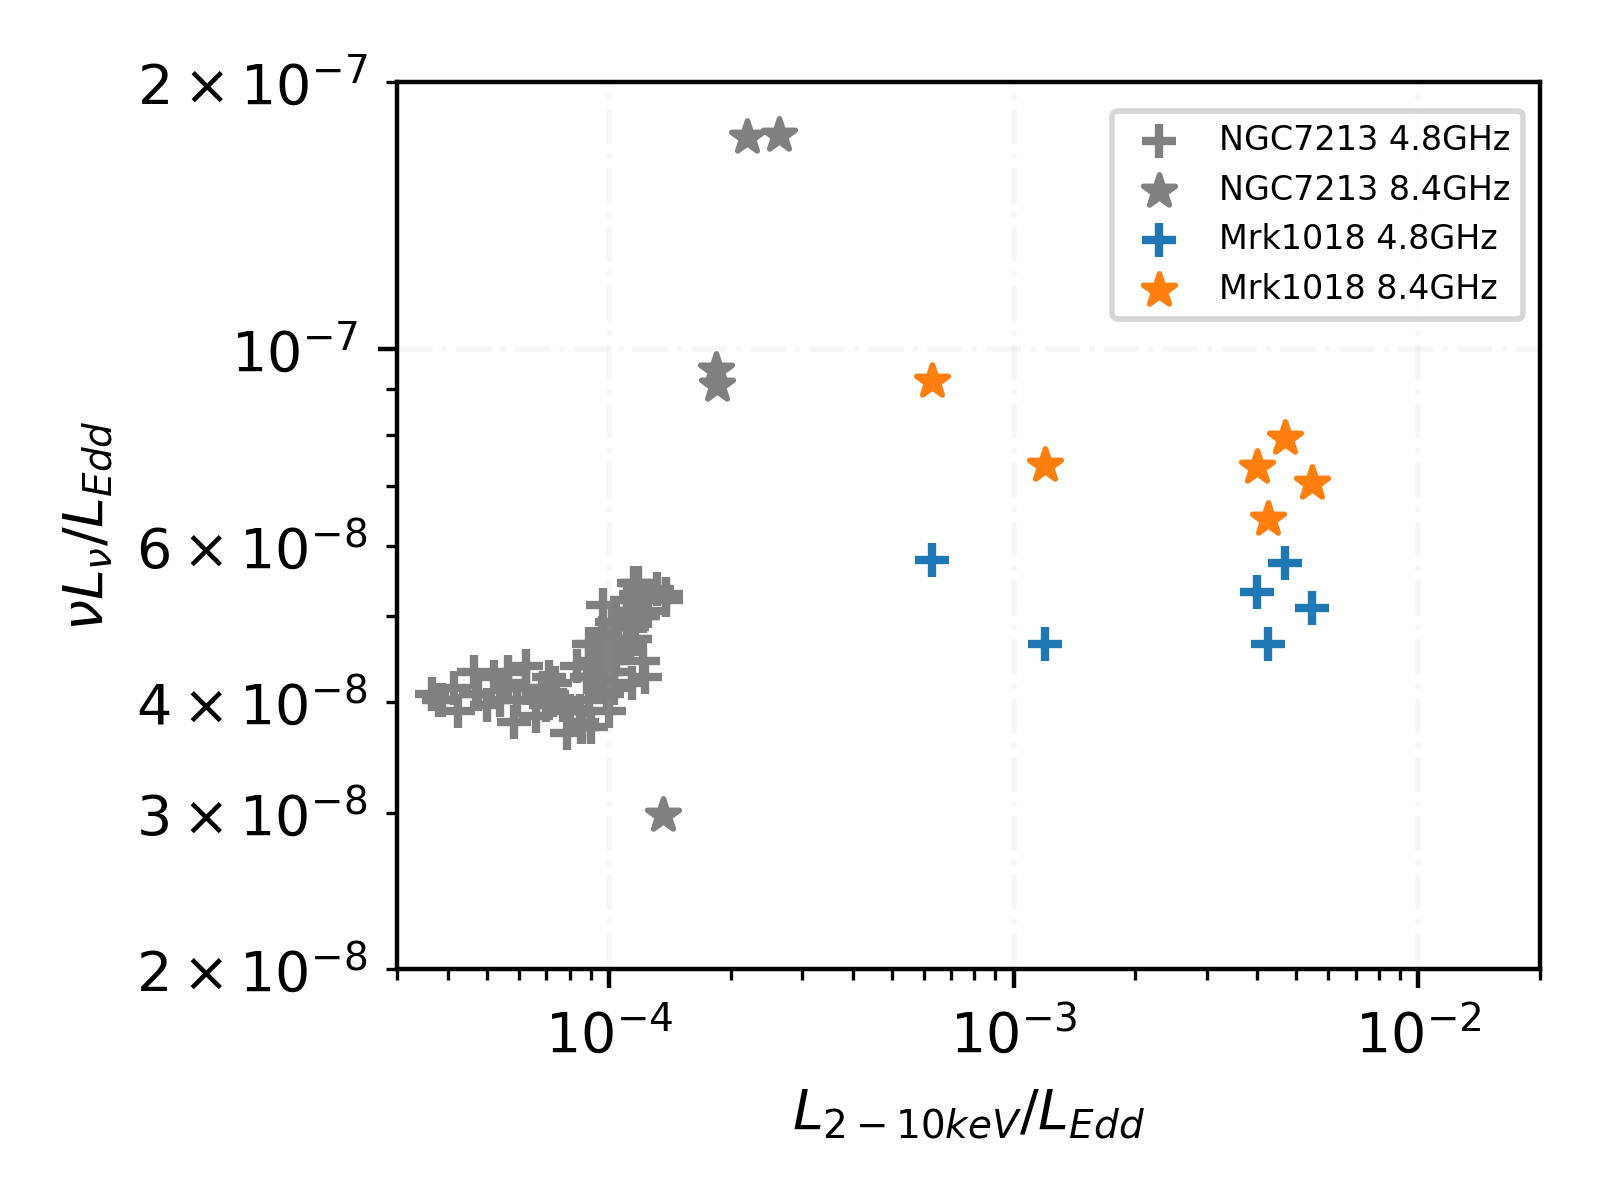
\includegraphics[width=0.9\textwidth]{./pic/Mrk1018_ngc7213_radio_xray_rate.png}
    \caption{Quasi-simultaneous $\nu L_{\nu}/L_{Edd}-L_{2-10keV}/L_{Edd}$ relation of Mrk1018}
    \label{fig:radio-xray-rate_relation_plus_ngc7213}
\end{figure}


\begin{figure}
\centering
	% To include a figure from a file named example.*
	% Allowable file formats are eps or ps if compiling using latex
	% or pdf, png, jpg if compiling using pdflatex
	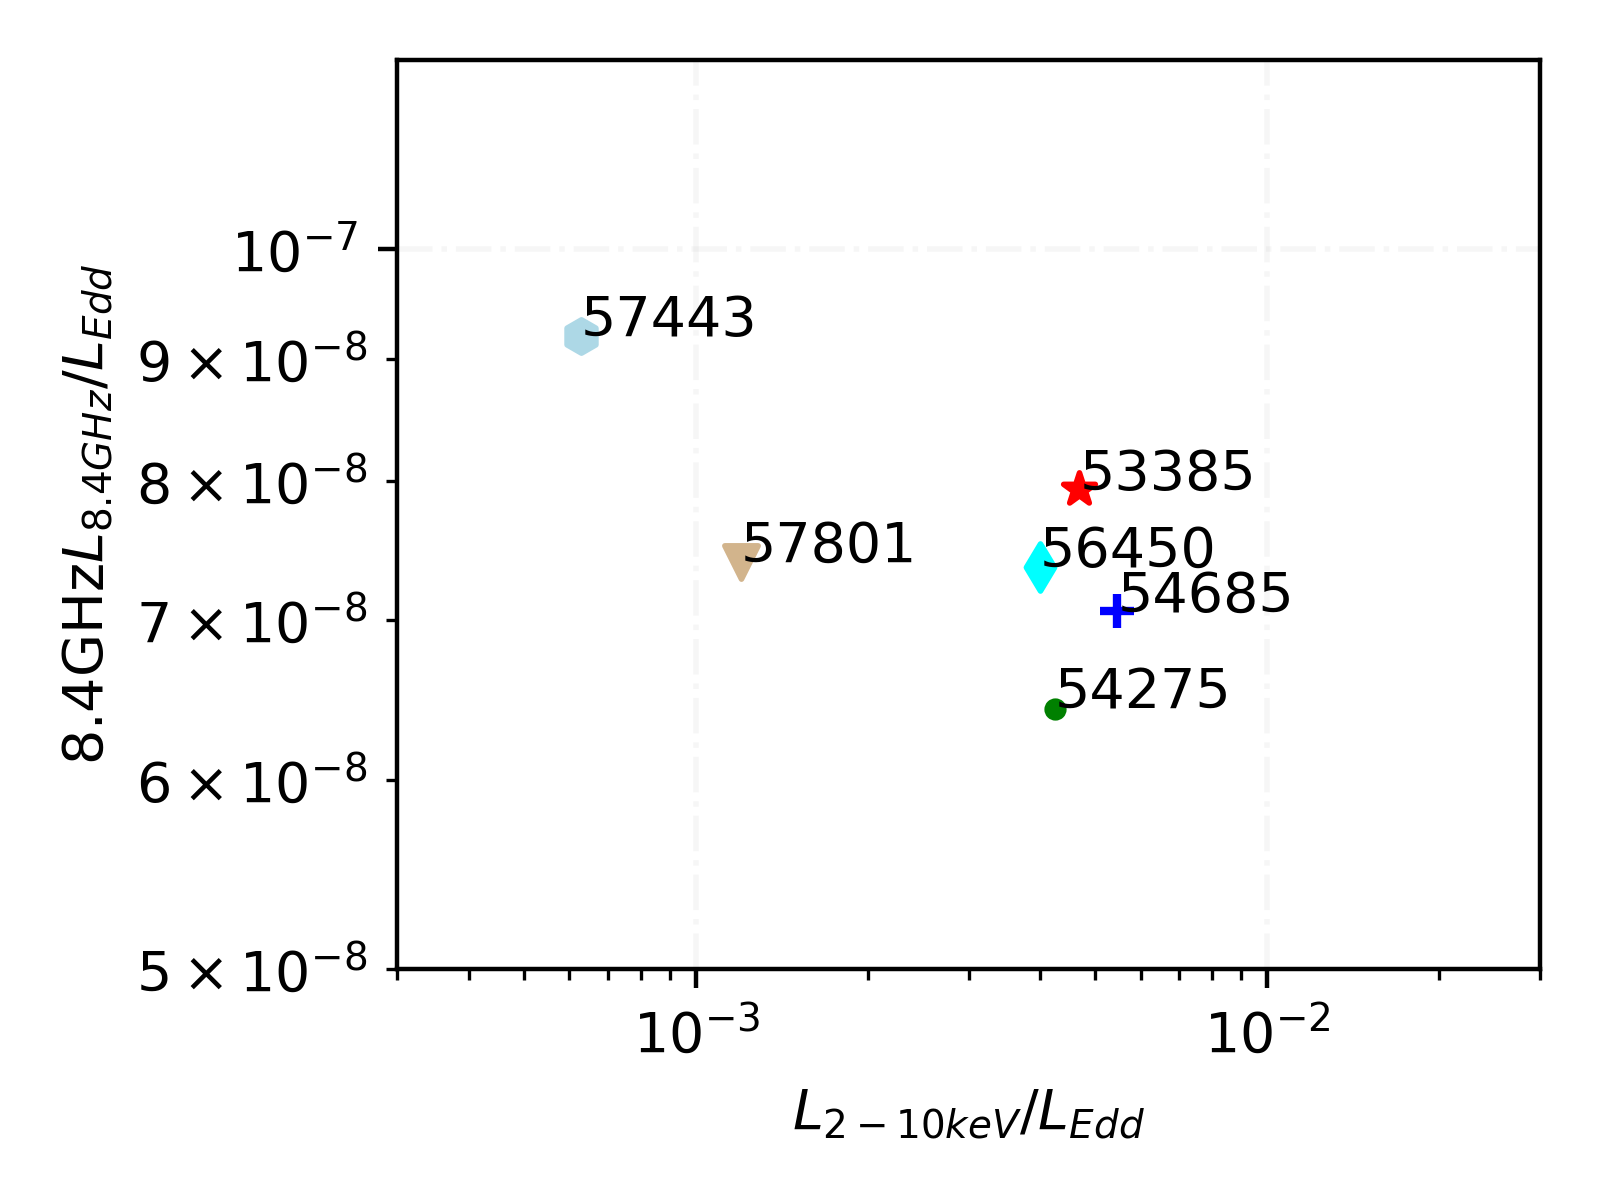
\includegraphics[width=0.9\textwidth]{./pic/Mrk1018_radio_xray_sel1_rate.png}
    \caption{Quasi-simultaneous $\nu L_{\nu}/L_{Edd}-L_{2-10keV}/L_{Edd}$ relation of Mrk1018}
    \label{fig:radio-xray-relation}
\end{figure}



\begin{figure*}
\centering
	% To include a figure from a file named example.*
	% Allowable file formats are eps or ps if compiling using latex
	% or pdf, png, jpg if compiling using pdflatex
	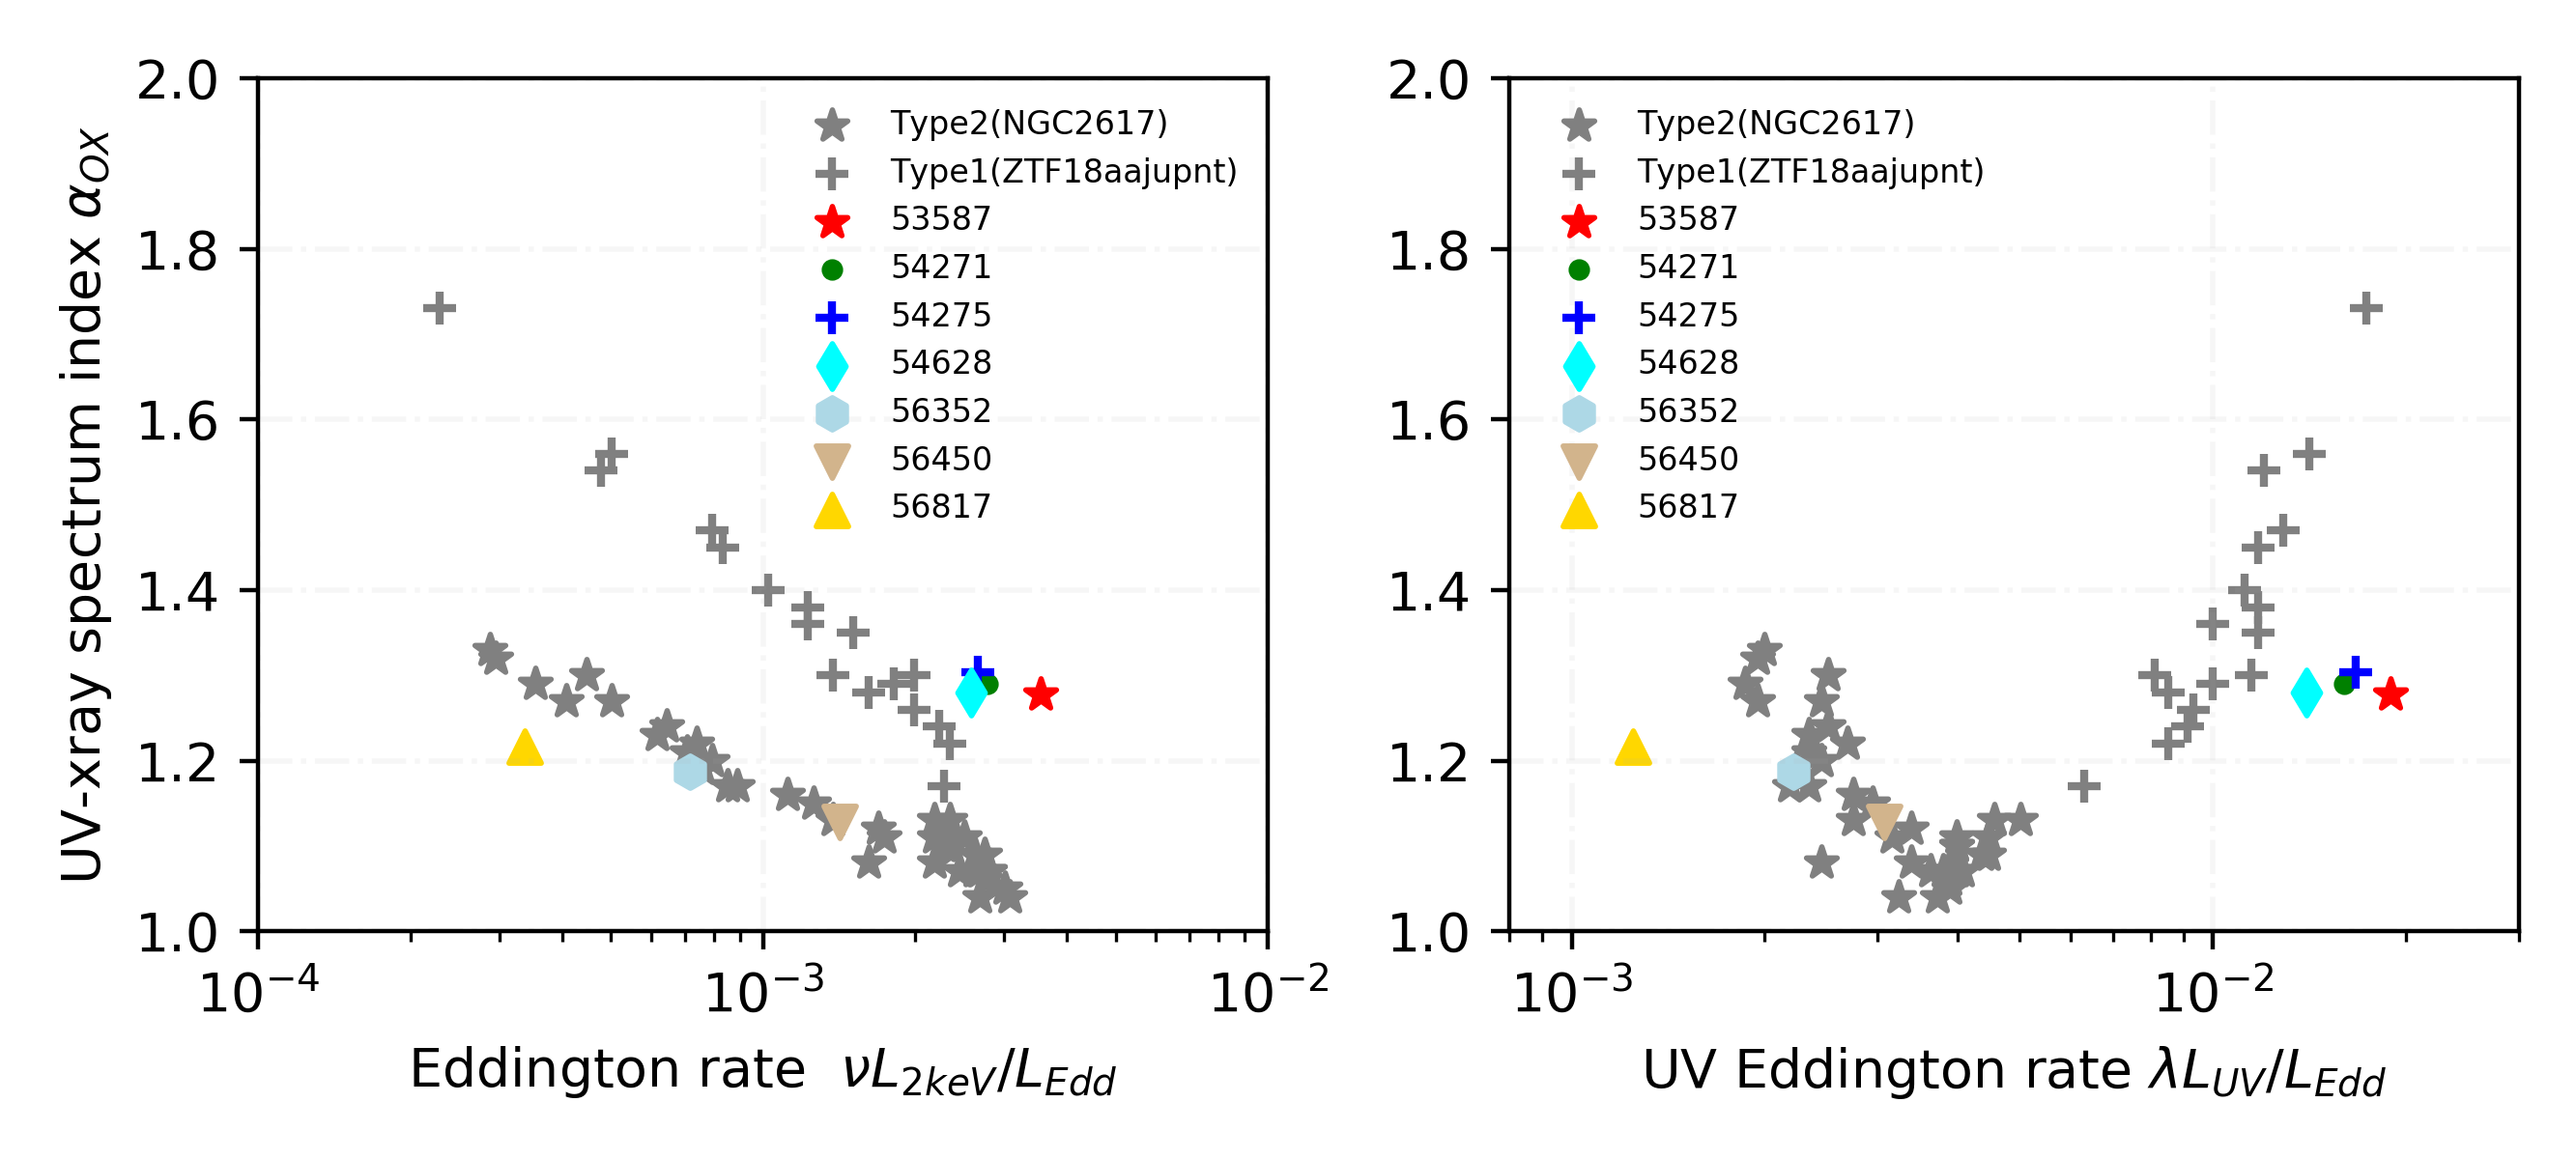
\includegraphics[width=0.9\textwidth]{./pic/Mrk1018_subplots_plus_2individuals_alpha_ox_L_x_Luv_rate.png}
    \caption{Mrk1018 and two other changing-look AGNs $\alpha_{OX}-\nu L_{2keV}/L_{Edd}$ and $\alpha_{OX}-\lambda L_{2500 \angstrom}/L_{Edd}$ diagram. Data of NGC~2617 and ZTF18aajupnt come from \citet{2019arXiv190904676R}.  }
    \label{fig:alpha_ox_luv}
\end{figure*}



\begin{comment}
Another tool we use to study the fractional variability is $F_{var}$ \citep[see ][]{2003MNRAS.345.1271V,2019ApJ...870..123E} defined as 
\begin{equation}
F_{var}=\sqrt{\frac{S^2-<\sigma^2_{err}>}{<x>^2}}
\end{equation}
where the variance of N data points is \begin{equation}
S^2=\frac{\sum_{i=1}^{N}{(<x>-x_i)^2}}{N-1}
\end{equation}
and the mean square error is \begin{equation}
<\sigma^2_{err}>=\frac{\sum_{i=1}^{N}{\sigma_{err,i}^2}}{N}
\end{equation}
We get $F_{var}$ for X-ray and U, UVW1, UVM2 and UVW2 band during this period as 23\%, 1.94\%, 6.08\%, 6.15\% and 5.93\%, respectively. 
\end{comment}



\begin{eqnarray}
F_\mathrm{2~keV}= 
\begin{cases}\frac{F_{2-10~ keV} (2-\Gamma)}{\nu_{2~keV} \times (5^{2-\Gamma}-1)},\quad \ \ & 
  \Gamma \neq 2 \\ 
  \frac{F_{2-10~ keV}}{\nu_{2~keV} \times \mathrm{ln} 5}, \quad \ \ & \Gamma = 2
\end{cases} 
\end{eqnarray}




\begin{comment}
\begin{equation}
F_\mathrm{\nu_1}=\frac{F_{\nu_1-\nu_2} (1-\alpha)}{\nu_1 \times ((\frac{\nu_2}{\nu_1})^{1-\alpha}-1)}
\end{equation} when $\Gamma \neq 2$ and
\begin{equation}
F_\mathrm{\nu_1}=\frac{F_{\nu_1-\nu_2}}{\nu_1 \times \mathrm{ln} \frac{\nu_2}{\nu_1}}
\end{equation} when $\Gamma = 2$. 
\end{comment}


    54926 & 2.29  $\pm$ 0.30  & 55015 & 10.00 $\pm$ 0.50  & -89   & 4.83E+38 & 4.21E+43 \\
    56550 & 2.63  $\pm$ 0.37  & 56450 & 7.90  $\pm$ 0.82  & 100   & 5.53E+38 & 3.33E+43 \\
    57481 & 2.56  $\pm$ 0.01  & 57443 & 1.27  $\pm$ 0.03  & 38    & 5.39E+38 & 5.35E+42 \\
    57768 & 2.07  $\pm$ 0.02  & 57801 & 2.44  $\pm$ 0.02  & -33   & 4.36E+38 & 1.03E+43 \\
    58087 & 1.97  $\pm$ 0.14  & 58123 & 2.10  $\pm$ 0.10  & -36   & 4.16E+38 & 8.85E+42 \\
    58472 & 2.83  $\pm$ 0.39  & 58445 & 0.70  $\pm$ 0.25  & 27    & 5.95E+38 & 2.96E+42 \\


\begin{figure*}
\centering
	% To include a figure from a file named example.*
	% Allowable file formats are eps or ps if compiling using latex
	% or pdf, png, jpg if compiling using pdflatex
	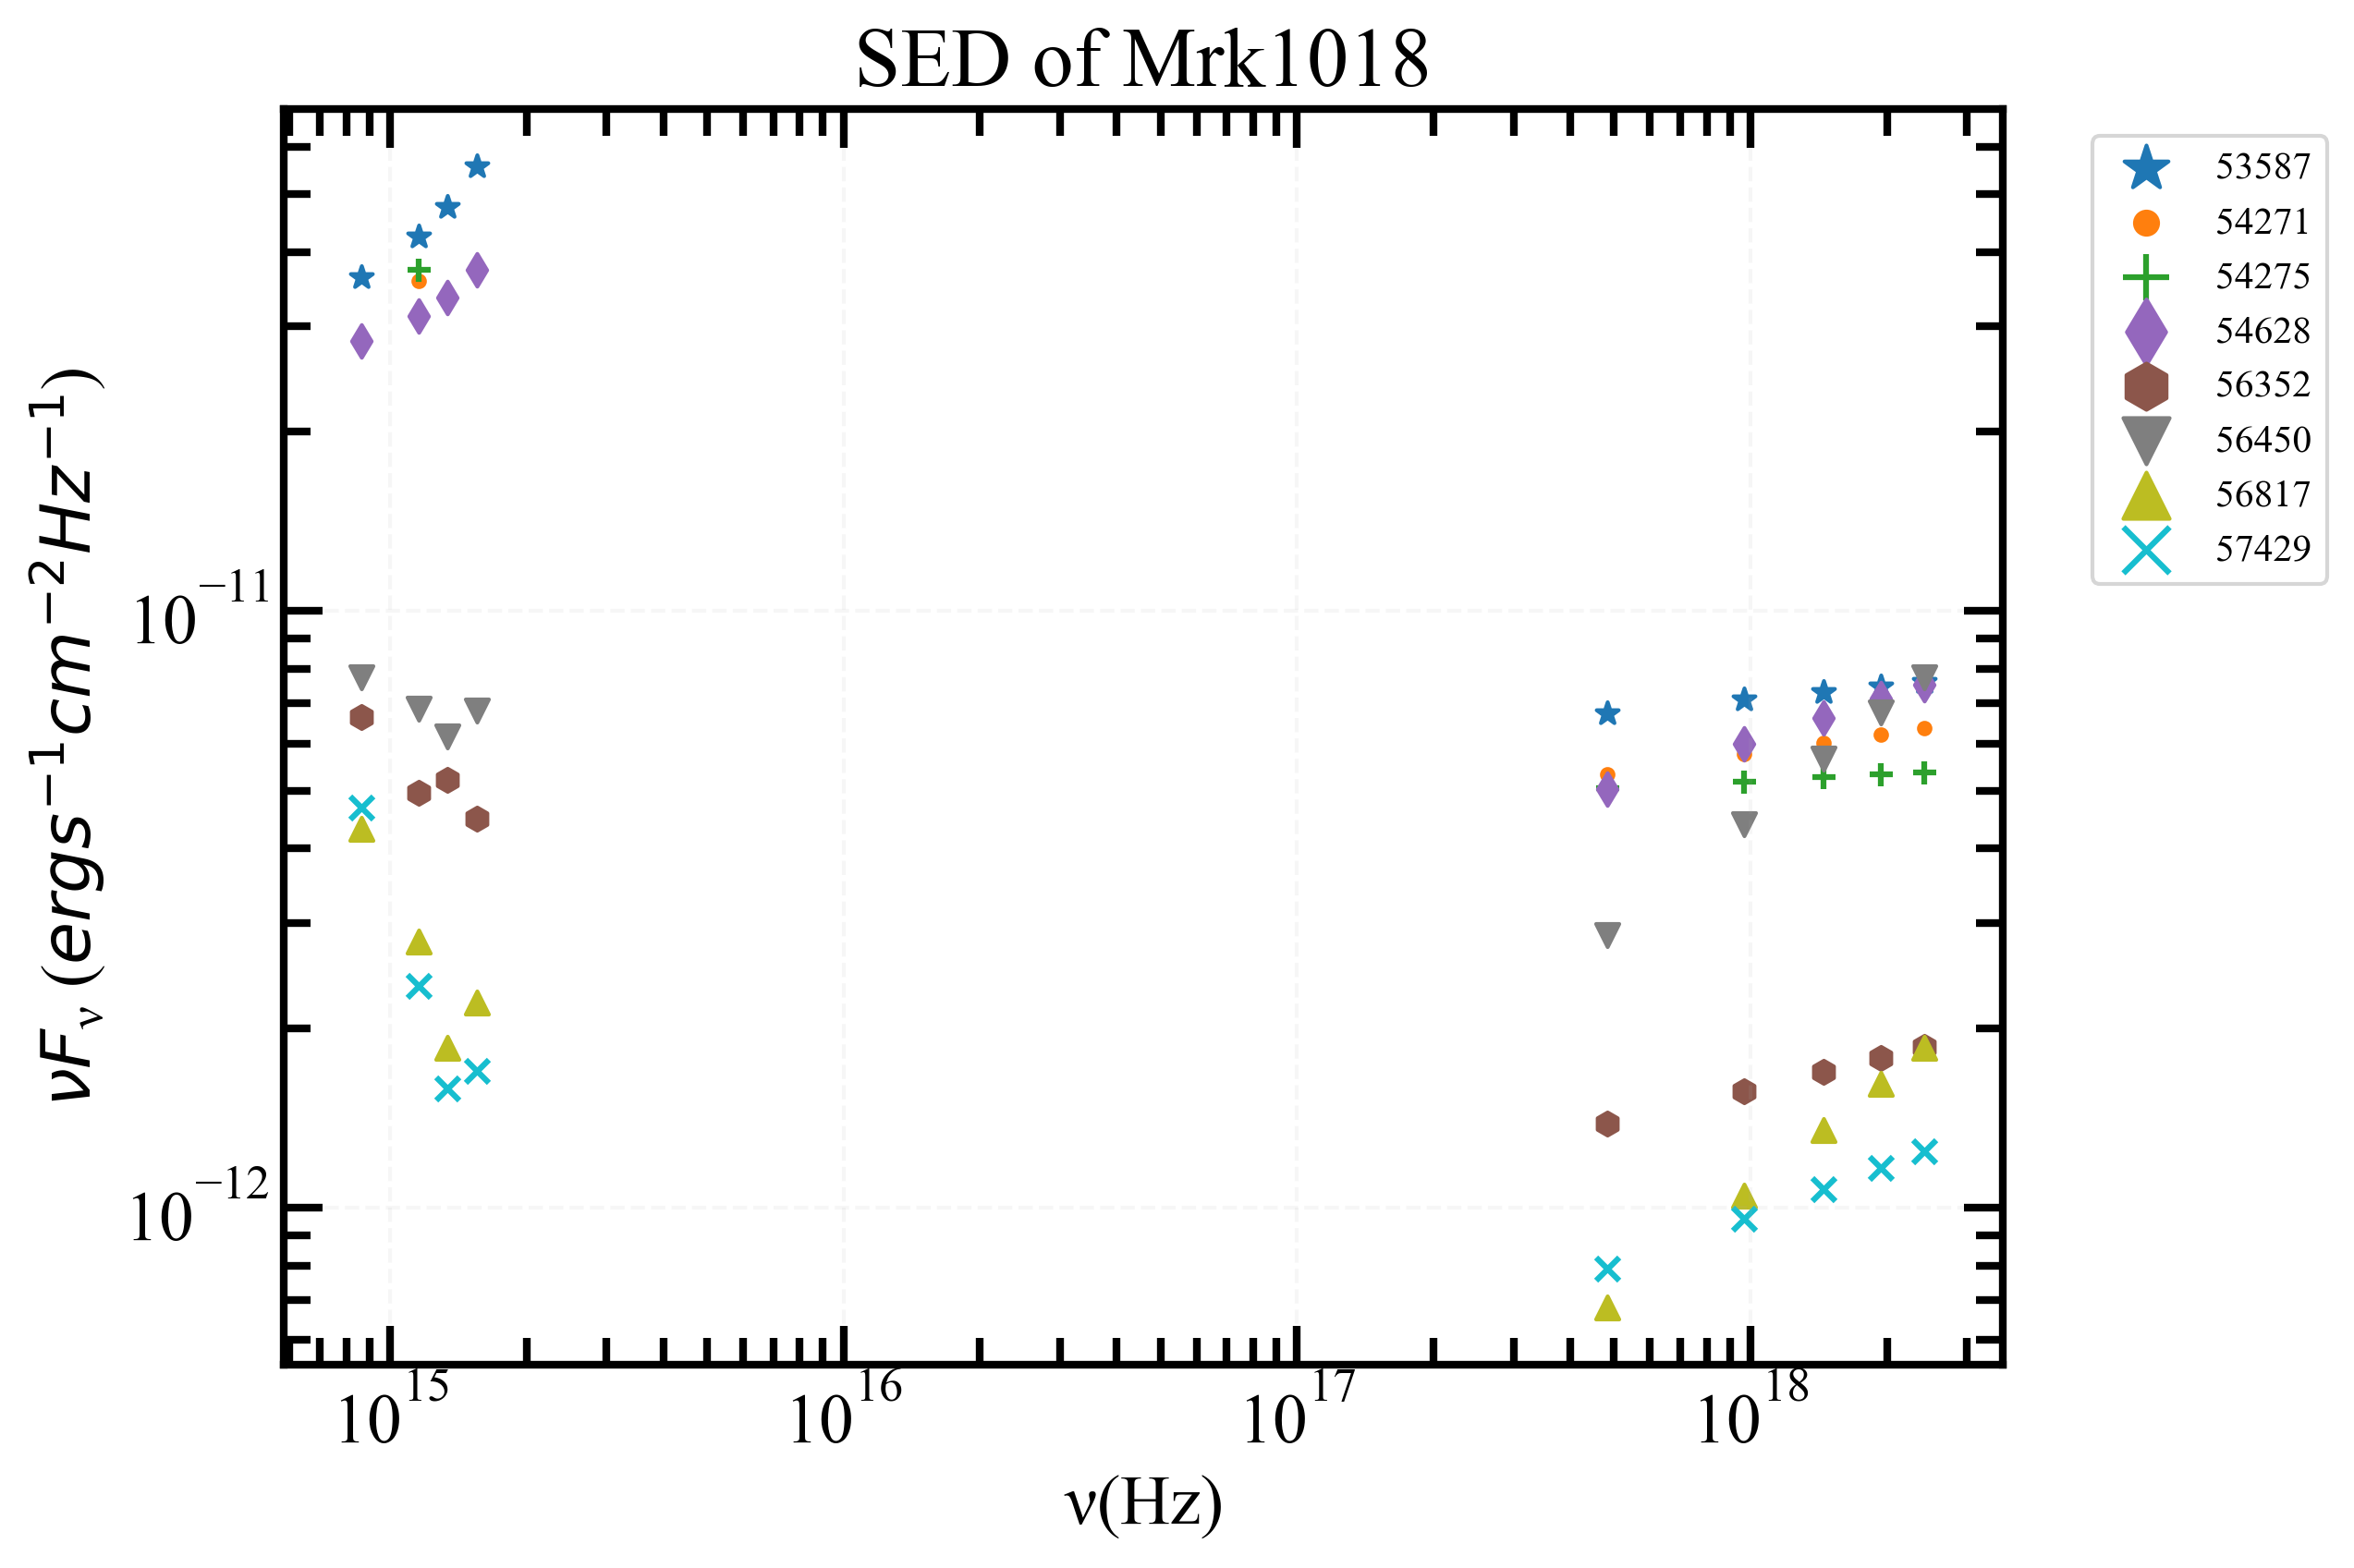
\includegraphics[width=0.8\textwidth]{./pic/Mrk1018_sed.png}
    \caption{SED between X-ray and ultraviolet. Red, green and blue markers correspond to type 1 phase, changing look phase and type 2 phase, respectively. }
    \label{fig:xray-uvot-sed}
\end{figure*}

%On the other hand, if the positive and negative correlation of $\Gamma$--$L_\mathrm{X}$ diagram found in AGNs and XRBs both associates with different type/state, Mrk~1018 in $\Gamma$--$L_\mathrm{X}$ diagram jumps from left branch to right branch within 98 days and return back to left branch within 367 days during a flare. 



The dynamic timescale is given as 
\begin{equation}
\tau_{dy} \sim (\frac{G M_\mathrm{BH}}{r^3})^{-1/2} \sim 5.7\times 10^{-3} (\frac{M_\mathrm{BH}}{10^8M_{\odot}})(\frac{r_d}{r_g})^{3/2} \, days
\end{equation} 

If we consider a disk radius of $r_d =100\, r_g$, and viscosity coefficient $\alpha=0.1$ , we can get a thermal timescale of $\sim$39 days, which is comparable to the flare timescale we find during the Changing-look phase.


%The discussion about whether the type transition on such short timescale is related to activeness of central engine or obscuration event is still continuing. 
%mechanism of type transition of CL AGNs through the multi-wavelength evolution.
%A tidal eruption event could not account for the Mrk 1018's type change. 


%...... (补充不同波段观测信息)
%

%An explanation of obscuration event for the variability is ruled out, since no intrinsic absorption in the X-ray spectrum is detected. It comes to the conclusion that change of type is consistent with declining accretion rate. \citet{2017A&A...607L...9K} reported the mini-outburst of Mrk~1018 in October 2016 with the brightening by a factor of 1.9 at least to February 2017. Far-UV continuum flux also increased by a factor of 1.5 in around one year during the outburst. It seems that radiation of corona and accretion disk comes from near region. We notice that Mrk~1018 has also experienced the re-brightening during the types transition period simultaneously in X-ray and UVOT band by a factor of $\sim3$ and $\sim1.3$, respectively, between 2013 Mar and 2013 Jun. With broad-band spectrum fitting in two states, \citet{2018MNRAS.480.3898N} suggests the drop of soft X-ray excess contributing most ionizing photons causes the disappearance of Broad Line Region(BLR) then the type transition. \citet{2018ApJ...861...51K} models the broad-line component with a recoiled super-massive black hole scenario with a $\sim$29 years orbital period and predicts that if the type transition repeats as past, it would occur again in mid-2020s. Before that, what the mechanism for such short-timescale light curve variability for AGN and type transition is remains unclear. 

%For this observation, the selection of source and background regions  are followed \citet{2017ApJ...840...11L}.  takes into account the pile-up effect with a JDPILEUP component and get the  $\Gamma =1.97_{+0.04}^{-0.03}$. It's similar to our result $\Gamma =2.02\pm{0.03}$ when we adopt the same pile-up model. \citet{2016A&A...593L...9H} excluded the brightest 9 pixels to avoid pile-up effects and get a lower $\Gamma =1.68\pm0.04$ determined from 4-8 keV range spectrum. The correction for pile-up effects will make the spectrum softer. \citet{2017A&A...607L...9K} ignored the pile-up effects and get a similar $\Gamma =1.7\pm0.03$ fitting in 0.5-8 keV. The fitting range selection will also influence the parameter $\Gamma$. So we adopt values from \citet{2017A&A...607L...9K} for the observation in 2010(MJD 55527).

%\subsection{Correlation between X-ray and Radio Luminosities}\label{subsec:xray-radio}
%We adopt data from intervals between X-ray and radio band as short as possible to explore the quasi-simultaneous flux in two bands. The correlation between the radio and X-ray flux is weak with a spearmanr coefficiency: -0.54, since the radio band flux of Mrk~1018 is flat relative to X-ray with a slope $\sim -0.1$ when fitting the non-linear relationship between $ L_\mathrm{R}$ and $ L_\mathrm{X}$ with log $L_\mathrm{R} \propto$ log $L_\mathrm{X-ray}$ , see also \autoref{fig:radio-xray-mass_relation_Plotkin2012}. 


%\subsection{Evolution of spectrum with Eddington rate}
%\label{subsec:g-f}
%We use the photon index ($\Gamma$) in X-ray and \alphaox ~ as probe to trace the relationship between corona and accretion disk during the type transition of Mrk~1018. 

 %We also calculated the \alphaox for only one observation during the type 2 AGN phase. 
%Only data before MJD 57434 is used for estimation of $\alpha_{OX}$. Based on all X-ray spectrum fit, we present the photon index evolution with flux and Eddington rate, as shown in \autoref{fig:xrayappendgood-fandg-tmap}. 


%With $\gamma \sim$ 1.5, we roughly get the slopes of $\alpha_{OX}$ on log $ L_{\mathrm{X}}$ and log $ L_\mathrm{UV}$ as  and , respectively (see also \autoref{fig:alpha_ox_lx_luv}).


%We also plot the relation between \alphaox and $L_\mathrm{bol}$ in Mrk 1018 (see \autoref{fig:alpha_ox_Lbol}), where the $L_\mathrm{bol}$ is simply taken as $30\times L_\mathrm{2-10keV}$ \citep{2009MNRAS.399..349G}. The best-fitting correlations between \alphaox and $L_\mathrm{bol}$ in the low luminosity AGNs \citep{2011ApJ...739...64X} and in the high luminosity AGNs \citep{2010A&A...512A..34L} are added in the plot. As the luminosity decreasing, Mrk 1018 transit from the positive correlation of the high luminosity branch to the negative correlation of the low luminosity branch. By analogy with the normal AGNs, the same mechanism behind the \alphaox--$L_\mathrm{bol}$ correlation also works in Mrk 1018, i.e. the SSD component weakens as the luminosity decreasing. 


%Mrk~1018 is located nearly at the transition between two accretion mode, with relatively flat slope in radio and X-ray Eddington rate $\nu L_{\nu}/L_{Edd}-L_{2-10keV}/L_{Edd}$ diagram.
%Mrk~1018 shows relatively flat radio-X-ray relation in the fundamental plane defined in \citet{2012MNRAS.419..267P}.


%%%%%%%%%%%%%%%%%%%%%%%%
%The different radio-X-ray slopes may be originated from different accretion mode (the slopes of 0.7 and 1.4 correspond to radiatively inefficient and radiatively efficient accretion flows, respectively, Coriat et al. 2011; Cao et al. 2014), or from the change of viscosity parameter $\alpha$ in a hot accretion flow (Xie \& Yuan 2016).
%%%%%%%%%%%%%%



%The evolution of X-ray photon index and $\alpha_{OX}$ with flux represents anti-positive/positive correlation in two branches (so called ``V-shape''). The V-shape both in $\Gamma-L_{2-10~keV}/L_{Edd}$ and $\alpha_{OX}-\lambda L_{2500\angstrom}/L_{Edd}$ diagram show much similarity with other changing-look AGNs \citep[see ][]{2019arXiv190904676R} and quasars \citep[see][]{2019ApJ...883...76R}. Unfortunately, there is a distinct flux gap between two branches for Mrk~1018 which could be caused by lack of observation during the transition period or two intrinsic separate states in Mrk~1018 and the type confirmation from optical spectrum is absent during the type transition phase (in 2013$\sim$2015). The feature in $\Gamma-L_{2-10~keV}/L_{Edd}$ diagram is also found in a large samples of normal AGNs. For example, \citet{2008ApJ...682...81S} finds significant and positive correlation between the hard X-ray photon index ($\Gamma$) and accretion rate ($L/L_{Edd}$) for moderate to high luminosity Radio-Quiet AGNs. The anti-positive correlation of $\Gamma-L_X/L_{Edd}$ in low-accreting AGNs is found with $10^{-10}\leq L_X/L_{Edd} \leq 10^{-3}$ and $10^{-6.5}\leq L_X/L_{Edd} \leq 10^{-3}$, \citep[see][]{2014MNRAS.443...72J,2015MNRAS.447.1692Y}, respectively, while positive correlation of $\Gamma-L_X/L_{Edd}$ is found when $L_X/L_{Edd} \geq 10^{-3}$ \citep[see][]{2015MNRAS.447.1692Y}. X-ray binaries and AGNs share similar anti-positive/positive correlation between X-ray photon index and Eddington ratio below/above a critical value of $L_{\rm bol}/L_{\rm Edd}\sim 10^{-2}$ \citep[e.g.,][and references therein]{2007ApJ...658..282Y,2008ApJ...682..212W,2009MNRAS.399..349G,2011A&A...530A.149Y,2015MNRAS.447.1692Y,2019arXiv191203971L,2019arXiv191212145Y}.

%The analogous of $\alpha_{OX}-L_{bol}/L_{Edd}$ in X-ray binaries and simulated AGNs spectral states compared to changing-look quasars is also found \citep[see ][]{2011MNRAS.417..280S,2011MNRAS.413.2259S,2019ApJ...883...76R}, which provides another link between stellar-mass black holes and super-massive black holes. As shown in Fig~\ref{fig:xrayappendgood-fandg-tmap} and ~\ref{fig:alpha_ox_luv}, we find that $\alpha_{OX}-\lambda L_{2500\angstrom}/L_{Edd}$ relation is well linked to the types of AGNs when compared with another two Changing-look AGNs.   

%What causes the two different branches in $\Gamma-L_{2-10~keV}/L_{Edd}$ diagram is unknown yet. A possible explanation with accretion mode transition has been suggested in Changing-look AGNs \citep[e.g.,][]{2019arXiv191200164A, 2019arXiv191203972L}, the low luminosity AGN (LLAGN) with large amplitude X-ray variability \citep[e.g.,][]{2019arXiv191201897L}, and BL Lac objects\citep[e.g.,][]{2003ApJ...599..147C} with analogous to X-ray binaries\citep[e.g.,][]{2005A&A...442L..15P,2018MNRAS.476.1581A}. If the accretion mode transition corresponds to the type transition, what mechanism makes it occur in such a short timescale is needed. 

%Whether the branches in $\Gamma-L_{2-10~keV}/L_{Edd}$ diagram correspond to the types of CL-AGNs is not for sure. But for normal AGNs, there is a random distribution in $\Gamma-L_X$ diagram for type 1 AGNs when luminosity range is large($\sim 1.78\times 10^{41}-1.53\times 10^{47} erg s^{-1} ; 4.5\times 10^{41}-9\times 10^{44} erg s^{-1}$) \citep[see][respectively]{1997MNRAS.286..513R,2015AASP....5...79S}, while \citet{2008AJ....135.1505S} shows strong and positive $\Gamma-L_X$ correlation in bright radio-quiet active galactic nuclei (AGNs) when type 1 and no-type 1 AGNs are divided into sub-samples with luminosity range from $10^{42}$ to $10^{45} erg s^{-1}$. It seems that anti-positive/positive correlation between $\Gamma$ and X-ray luminosity or Eddington rate below/above the so-called critical accretion rate mainly relies on luminosity and radio properties no matter what the type of AGNs are. \citet{2008ApJ...682...81S} finds that $\alpha_{OX}$ relies on optical-UV luminosity, in radio-quiet (RQ) active galactic nuclei (AGNs), rather than $L_{Bol}/L_{Edd}$, consistent with \citet{2012MNRAS.423..600S} in type 1 AGNs where optical-UV luminosity mainly drives the X-ray to UV emission ratio, rather than $M_{BH}$ or $L_{Bol}/L_{Edd}$. So it might be $L_{X}$ and $L_{UV}$ that drives $\Gamma$ and $\alpha_{OX}$ in two branches, respectively.

%The 2--10~keV flux variability reaches a factor around 8--10 between 2009 and 2016, which is consistent with the dimming of the central engine with zero intrinsic absorption. 

%\citet{2014MNRAS.438.3340E} describes a evolutionary sequence that the AGN type evolution sequence:type 1 $\to$ 1.2/1.5 $\to$ 1.8/1.9 $\to$ 2 as luminosity (or accretion rate onto black hole) decreases in a disc-wind scenario for broad line region. It's consistent with the type evolution of Mrk~1018, despite of lack of optical confirmation in middle type. 

%$\alpha_{OX}-\lambda L_{2500\angstrom}/L_{Edd}$ relation consistent with another two CL-AGNs supports that the decrease of $L_{UV}$ drives the type transition of Mrk~1018.


%If Mrk 1018 follows ``hybrid" correlation, it would follow the standard correlation below the critical luminosity, since the two data at left end (with lowest X-ray luminosities) roughly agree with the best-fitting line. \citet{2018MNRAS.473.4122E} find that the radio spectral indices of the samples in the standard branch (with slope $\sim 0.6$) are systematically higher than the outliers.


%For $M=10^{8} M_{\odos}$, $R=10R_{s}$, Timescale	for	hot	gas	to	accrete	to	the	BH, $t_{acc}\sim(1/\alpha \Omega)(R/H)^{2}\sim 5 days$.		

 % Some studies have drew an analogy between the changing-look AGN and the Galactic BH X-ray transits \citep[e.g. ][]{2018MNRAS.480.3898N,2019ApJ...883...76R}. The decay timescale of an outburst of a BH X-ray transit roughly corresponds to the viscous timescale of outer disk \citep[e.g. ][]{1998MNRAS.293L..42K}. Scaling to a $10^{8}M_{\odot}$ BH, the viscous timescale is roughly one million years \citep{2012MmSAI..83..469L,2018MNRAS.475.1190Y}, which is much longer than characteristic decay timescale we got in Mrk 1018. So the declining of the luminosity of Mrk 1018 can not be controlled by the viscous process of the outer disk \citep[see also ][]{2018MNRAS.480.3898N}. 
 
 
% Radiation pressure instability plus inner optically thin Advection-Dominated Accretion Flow \citep[see][]{2019arXiv190406767S} provides a possible explanation of outbursts of Changing-look AGN. 

%$t_{decay}=\frac{\Sigma \Delta R 2\pi R}{\dot{M}}$

%magnetically elevated accretion  \citep[see][]{2019MNRAS.483L..17D} 

%$t_{inflow}$ 
 
 
% The correlation between the optical and X-ray fluxes during the decay phase, which might correspond to near radiation region  between X-ray corona and accretion disk, as also suggested in \citet{2017A&A...607L...9K}. We need monitor the multi-band light curve with higher frequency to estimate the time delay of radiation from X-ray and UV/optical.


%DIM, thermal-viscous disk instabilities timescale in X-ray binaries and AGNs \citep[e.g.,][for details and reviews)]{2001NewAR..45..449L,2009A&A...496..413H,2019arXiv191001852H}
%$t_{dim} $


%{2015ApJ...805...87Y,2015ApJ...811...23Y}

%Several typical characteristic timescale with viscosity parameter $alpha=0.1$ suggested in \citet{2018MNRAS.480.3898N}:

%$t_{dyn}\sim (\frac{GM_{BH}}{R^3})^{-\frac{1}{2}} \sim $4 days

%$t_{thermal}\sim \frac{t_{dyn}}{\alpha}\sim $ 1 month

%$t_{visous}\sim \frac{t_{dyn}}{\alpha}\,(\frac{H}{R})^{-2}\sim $ $4 \times 10^5$years


%and references therein
%e.g.,






%\subsection{Summary}
%\begin{enumerate}
%\item The flux in X-ray and UV bands roughly declines by a factor of 20 and 9 within several years, during which the spectral type of AGN changes from type 1 to type 2. However, the radio flux only varies by a factor less than 2, in $\sim$15 years. 

%\item The X-ray and UV fluxes also show short-term variability with a timescale is as short as $\sim$ 100-400 days with a factor of $\sim$3--4 during the type transition phase and several days with a factor of 3 in faint state???.

%\item The $\Gamma-L_{X}$ diagram both appear as ``V-shape''. 
%\end{enumerate}

%The severe variability of Mrk~1018 in short timescale provides a good target for intrinsic activity of individual Super-massive Black Holes(SMBH). Considering all observational evidence, we can draw a full picture about how Mrk~1018's spectrum evolves with luminosity. As the luminosity declines, both corona and accretion disk varies. The decay timescale indicates that the variability of X-ray is relative to the thermal and dynamical process.  Furthermore, we need to explore more CL-AGNs and compare them to XRBs and normal AGNs in order to verify the mechanism of rapid variability.  

\footnote{Since the fluxes of the six filters of UVOT are all dominated by the host galaxy after $\sim$ MJD 57429.}